\documentclass[11pt]{article} 
\usepackage[english]{babel}
\usepackage[utf8]{inputenc}
\usepackage[margin=0.5in,top=0.5in,bottom=0.75in]{geometry}
\usepackage{amsmath}
\usepackage{amsthm}
\usepackage{amsfonts}
\usepackage{amssymb}
\usepackage[usenames,dvipsnames]{xcolor}
\usepackage{graphicx}
\usepackage[siunitx]{circuitikz}
\usepackage{tikz}
\usepackage[colorinlistoftodos, color=orange!50]{todonotes}
\usepackage{hyperref}
\usepackage[numbers, square]{natbib}
\usepackage{fancybox}
\usepackage{epsfig}
\usepackage{soul}
\usepackage[framemethod=tikz]{mdframed}
\usetikzlibrary{positioning, automata, backgrounds}
\usepackage{tikz}\usetikzlibrary{arrows.meta,backgrounds,calc,quotes}
\usepackage[shortlabels]{enumitem}
\usepackage[version=4]{mhchem}
\usepackage{multicol}
\usepackage{forest}
\usepackage{mathtools}
\usepackage{comment}
\usepackage{enumitem}
\usepackage[utf8]{inputenc}
% \usepackage[linesnumbered,ruled,vlined]{algorithm2e}
\usepackage{algorithm}
\usepackage[noend]{algpseudocode}
\usepackage{listings}
\usepackage{color}
\usepackage[numbers]{natbib}
% \usepackage{algorithm}
\usepackage{subfiles}
\usepackage{tkz-berge}


\newtheorem{prop}{Proposition}[section]
\newtheorem{thm}{Theorem}[section]
\newtheorem{lemma}{Lemma}[section]
\newtheorem{cor}{Corollary}[prop]
\DeclarePairedDelimiter\ceil{\lceil}{\rceil}
\DeclarePairedDelimiter\floor{\lfloor}{\rfloor}

\theoremstyle{definition}
\newtheorem{definition}{Definition}

\theoremstyle{definition}
\newtheorem{required}{Problem}
\newtheorem*{requiredHC}{Problem HC}

\theoremstyle{definition}
\newtheorem{ex}{Example}

\newcommand{\interval}[4]{\draw (#2, #1) -- (#3, #1); % Usage: \interval{height}{start}{end}{label}
\draw (#2, #1-0.11) -- (#2, #1+0.11); % draw left whisker
\draw (#3, #1-0.11) -- (#3, #1+0.11); % draw right whisker
\node[] at (#2-0.25, #1) {#4};
}

\tikzset{>={Stealth[length=7pt]}}
\tikzset{
    vertex/.style={circle,draw,minimum size=16,inner sep=0pt,font=\normalsize},
    edgelabel/.style={rectangle,draw=none,font=\footnotesize,outer sep=0pt},
    every node/.style={vertex},
    every edge quotes/.append style={edgelabel},
    every to/.append style={every node/.style={edgelabel}},
    wide/.style={line width=4pt,>={Stealth[length=18pt]}},
    directed/.style={arrows={->},font=\small},
    caption/.style={text width=6cm,align=center,rectangle,draw},
}


\setlength{\marginparwidth}{3.4cm}
%#########################################################

%To use symbols for footnotes
\renewcommand*{\thefootnote}{\fnsymbol{footnote}}
%To change footnotes back to numbers uncomment the following line
%\renewcommand*{\thefootnote}{\arabic{footnote}}

% Enable this command to adjust line spacing for inline math equations.
% \everymath{\displaystyle}

% _______ _____ _______ _      ______ 
%|__   __|_   _|__   __| |    |  ____|
%   | |    | |    | |  | |    | |__   
%   | |    | |    | |  | |    |  __|  
%   | |   _| |_   | |  | |____| |____ 
%   |_|  |_____|  |_|  |______|______|
%%%%%%%%%%%%%%%%%%%%%%%%%%%%%%%%%%%%%%%

\title{
\normalfont \normalsize 
\textsc{CSCI 3104 Fall 2022 \\ 
Instructors: Prof. Grochow and Nagesh} \\
[10pt] 
\rule{\linewidth}{0.5pt} \\[6pt] 
\huge Problem Set 7 \\
\rule{\linewidth}{2pt}  \\[10pt]
}
%\author{}
\date{}

\begin{document}

\definecolor{processblue}{cmyk}{0.96,0,0,0}
\definecolor{processred}{rgb}{200, 0, 0}
\definecolor{processgreen}{rgb}{0, 255, 0}
\DeclareGraphicsExtensions{.png}
\DeclareGraphicsExtensions{.gif}
\DeclareGraphicsExtensions{.jpg}

\maketitle


%%%%%%%%%%%%%%%%%%%%%%%%%
%%%%%%%%%%%%%%%%%%%%%%%%%%
%%%%%%%%%%FILL IN YOUR NAME%%%%%%%
%%%%%%%%%%AND STUDENT ID%%%%%%%%
%%%%%%%%%%%%%%%%%%%%%%%%%%
\noindent
Due Date \dotfill October 24, 2022 \\
Name \dotfill \textbf{Tyler Huynh} \\
Student ID \dotfill \textbf{109603994} \\
Collaborators \dotfill \textbf{List Your Collaborators Here}

\renewcommand{\thesubsection}{\arabic{section}(\alph{subsection}). }

\tableofcontents

\section*{Instructions}
\addcontentsline{toc}{section}{Instructions}
 \begin{itemize}
	\item The solutions \textbf{must be typed}, using proper mathematical notation. We cannot accept hand-written solutions. Useful links and references on \LaTeX can be found \href{https://canvas.colorado.edu/courses/75824/pages/latex}{here on Canvas}.
	\item You should submit your work through the \textbf{class Canvas page} only. Please submit one PDF file, compiled using this \LaTeX \ template.
	\item You may not need a full page for your solutions; pagebreaks are there to help Gradescope automatically find where each problem is. Even if you do not attempt every problem, please submit this document with no fewer pages than the blank template (or Gradescope has issues with it).

	\item You are welcome and encouraged to collaborate with your classmates, as well as consult outside resources. You must \textbf{cite your sources in this document.} \textbf{Copying from any source is an Honor Code violation. Furthermore, all submissions must be in your own words and reflect your understanding of the material.} If there is any confusion about this policy, it is your responsibility to clarify before the due date. 

	\item Posting to \textbf{any} service including, but not limited to Chegg, Reddit, StackExchange, etc., for help on an assignment is a violation of the Honor Code.

	\item You \textbf{must} virtually sign the Honor Code (see Section \hyperlink{HonorCode}{Honor Code}). Failure to do so will result in your assignment not being graded.
\end{itemize}


\section*{Honor Code (Make Sure to Virtually Sign the Honor Pledge)} 
\addcontentsline{toc}{section}{Honor Code (Make Sure to Virtually Sign the Honor Pledge)}
\hypertarget{HonorCode}{}

\begin{requiredHC}
On my honor, my submission reflects the following:
\begin{itemize}
\item My submission is in my own words and reflects my understanding of the material.
\item Any collaborations and external sources have been clearly cited in this document.
\item I have not posted to external services including, but not limited to Chegg, Reddit, StackExchange, etc.
\item I have neither copied nor provided others solutions they can copy.
\end{itemize}

\noindent In the specified region below, clearly indicate that you have upheld the Honor Code. Then type your name. 
\end{requiredHC}

\begin{proof}[Honor Pledge]
I, \textbf{Tyler Huynh} on my honor pledge that my submission is a reflection of my own understanding of the material, any and all collaborations/sources have been properly cited, I have not posted any material to external sources, and I have not copied other solutions as my own.
\end{proof}



\newpage
\setcounter{section}{18}
\section{Standard 19 - Solving Recurrences: Tree Method}

\setcounter{required}{18}
\begin{required} 
Consider the recurrence $T(n)$ below. Using the {\bf tree method}, determine a suitable function $f(n)$ such that $T(n) \in \Theta(f(n))$. Clearly show all steps. Note the following:
\begin{itemize}
\item You may assume, without loss of generality, that $n$ is a power of $3$ (i.e., $n = 3^{k}$ for some integer $k \geq 0$).
\item You may hand-draw your tree and embed it, provided it is legible and we do not have to rotate our screens to read it. However, \textbf{all your calculations must be typed}.
\end{itemize}

\[
T(n) = \begin{cases} 1, &  n < 3 \\ 
9T(n/3) + n^{2}, &  \text{otherwise.} \end{cases}
\]

\end{required}

\begin{proof}[Answer]
I will first begin by finding how many times we reach the base case of k: \\
\begin{align*}
\frac{n}{3^k}  &< 3\\
\log_3 n &< \log_3 (3^k, 3) \\
\log_3 n&< k + \log_3 3 \\
k &> \log_3 n - \log_3 3  \\
k &> \log_3 n - 1
\end{align*}
From the above we see that this will be the amount of time it will run, until we reach the base case of k.\\

I will now find the tree of T(n): \\
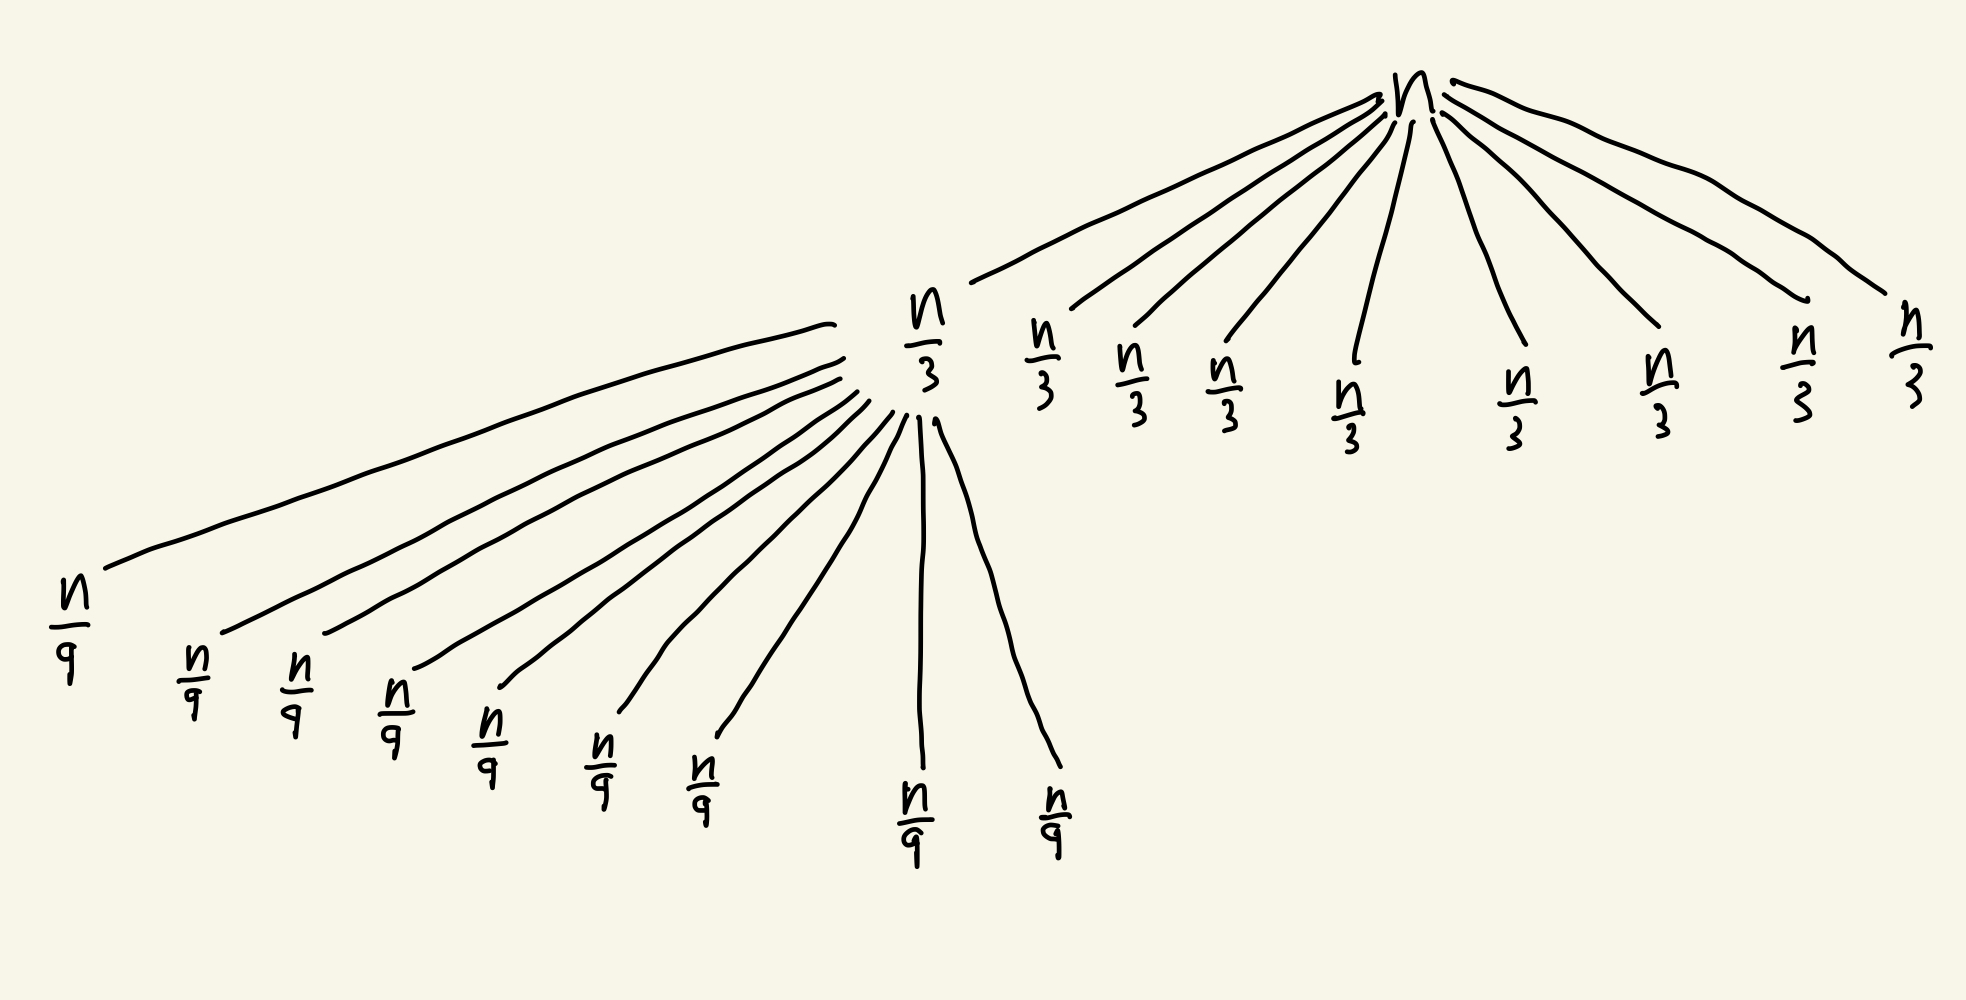
\includegraphics[width=0.6\textwidth]{IMG_F40695BF3954-1.jpeg}\\
From the above for the children of $\frac{n}{3}$ will have 9 children, that will have a value $\frac{n}{9}$. \\

I will now find T(n):\\
\begin{align*}
T(n) &= \textrm{(cost of base case) · (number of times the base case is reached)} + \sum_{i=0}^{\log_3 n - 1}  9^{i} * (\frac{n}{3^i})^2 \\
&= 9^k * 1 + \sum_{i=0}^{\log_3 n - 1}  9^{i} * (\frac{n}{3^i})^2 \\
&= 9^k + \sum_{i=0}^{\log_3 n - 1}  9^{i} * \frac{n^2}{3^{2i}}\\
&= 9^k + \sum_{i=0}^{\log_3 n - 1}  9^{i} * \frac{n^2}{9^i}\\
&= 9^k + n^2 * (\log_3 n - 1) \\
&= 9^k + n^2\log_3 n - n^2 \\
&= 9^{\log_3 n - 1} + n^2\log_3 n - n^2 \\
&= \frac{9^{\log_3 n}}{9} + n^2\log_3 n - n^2 \qquad \textrm{Log base change:} \qquad 9^{\log_3 n - 1} = \frac{\log_9 n}{\log_9 3}\\
&= \frac{9^{\frac{\log_9 n}{\log_9 3}}}{9} + n^2\log_3 n - n^2 \\
&= \frac{9^{\frac{\log_9 n}{1/2}}}{9} + n^2\log_3 n - n^2 \\
&= \frac{9^{2\log_9 n}}{9} + n^2\log_3 n - n^2 \\
&= \frac{9^{\log_9 n^2}}{9} + n^2\log_3 n - n^2 \\
&= \frac{n^2}{9} + n^2\log_3 n - n^2 \\
T(n) &= \Theta(n^2\log n)
\end{align*}
From the above we can see that the largest component would be $(n^2\log n)$, such that our final runtime complexity of T(n) will be: \\
\begin{center}
$T(n) = \Theta(n^2\log n)$
\end{center}
\end{proof}

\newpage
\section{Standard 20 - QuickSort}

\begin{required} \label{unrolling}
\begin{enumerate}[label=(\alph*)]
\subsection{Part \ref{S20a}}

\item \label{S20a} Write down a recurrence relation that models the {\bf best case} running time of Quicksort, i.e. the case where {\sc Partition} selects the {\bf median} element at each iteration. What is the best-case running time of QuickSort? Be sure to write \textbf{both the recurrence relation and the runtime.}

\begin{proof}[Answer] \textbf{Referenced Levet notes} \\
% YOUR ANSWER BELOW
Our recurrence relation below: \\
\begin{align*}
T(n) = \begin{cases}
\Theta(1) & : n \leq 2, \\
2T(\frac{n}{2}) + \Theta(n) & : n > 2.
\end{cases}
\end{align*}

The best-case running time of QuickSort is.... when the algorithm chooses the median in a list as the pivot, i.e. also splitting it in half. Below I will show how I come to this conclusion: \\

I will solve my recurrence relation to find the runtime of T(n) by using the tree method: \\
I will first begin by finding how many times until we reach the base case of k: \\
\begin{align*}
\frac{n}{2^k} &\leq 2 \\
\log_2 n &\leq \log_2 (^k, 2) \\
\log_2 n &\leq k + \log_2 2 \\
k &\geq \log_2 n - \log_2 2 \\
k &\geq \log_2 n - 1
\end{align*}

From the above we see that this will be the amount of times it will run, until we reach the base case of k. \\
I will now find the tree of T(n): \\
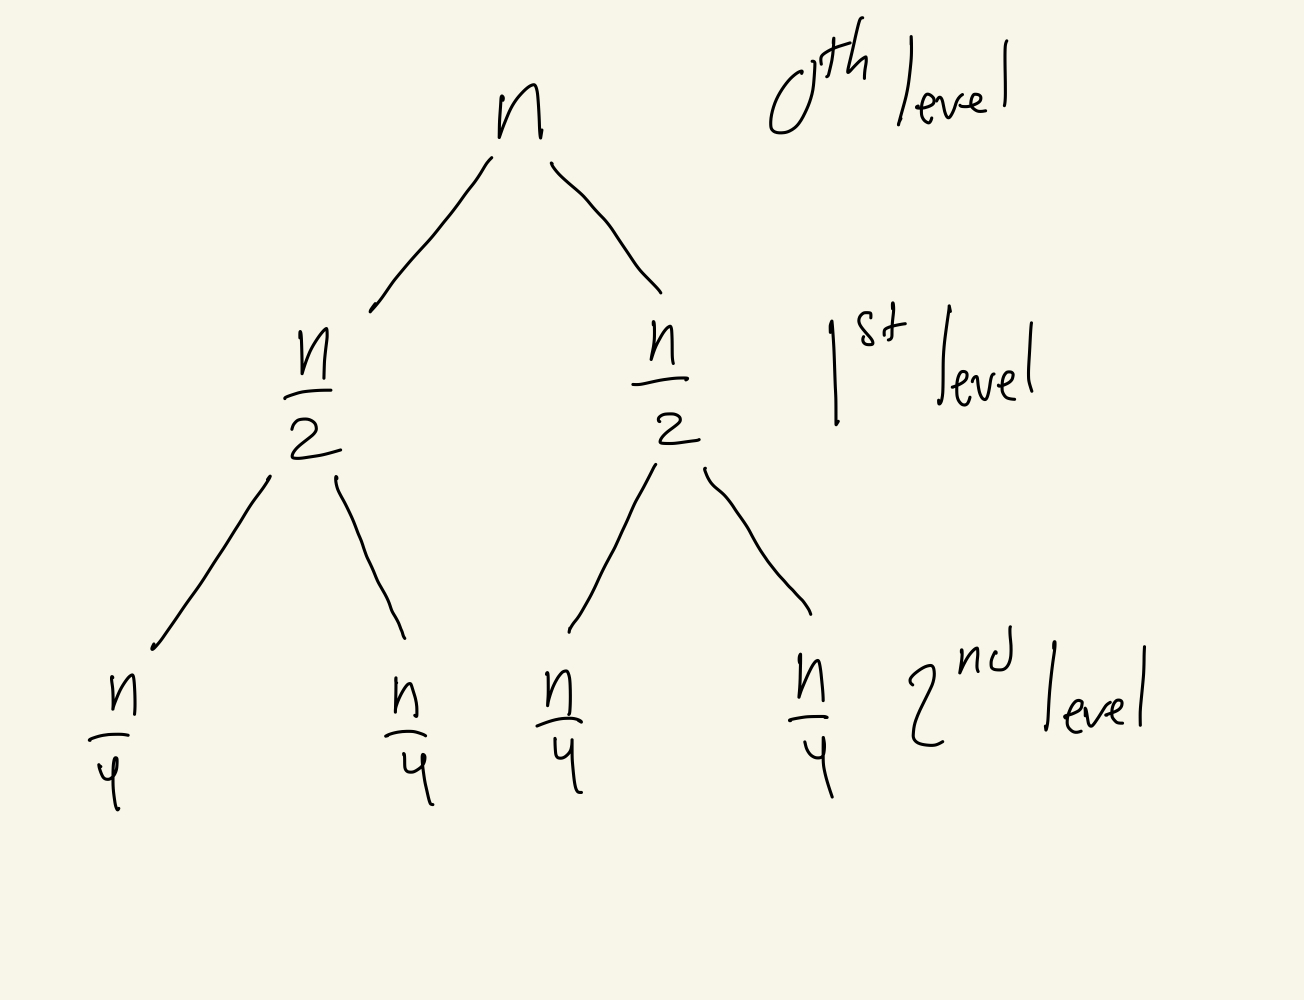
\includegraphics[width=0.6\textwidth]{IMG_D7646ABE293A-1.jpeg}\\

I will now solve for T(n): \\
\begin{align*}
T(n) &= \textrm{(cost of base case) · (number of times the base case is reached)} + \sum_{i=0}^{\log_2 n - 1}  2^{i} * \frac{n}{2^i} \\
&= \Theta(1) * 2^k +  \sum_{i=0}^{\log_2 n - 1}  2^{i} * \frac{n}{2^i} \\
&= \Theta(1) * 2^{\log_2 n-1} + \sum_{i=0}^{\log_2 n - 1}  n \\
&= \Theta(1) * 2^{\log_2 n-1} + n(\log_2 n - 1) \\
&= \Theta(1) * 2^{\log_2 n-1} + n\log_2 n - n \\
&= \Theta(1) * 2^{\log_2 n} * 2^-1 + n\log_2 n - n \\
&= \Theta(1) * n * \frac{1}{2} *  n\log_2 n - n \\
&= \frac{\Theta(1)}{2} + n\log_2 n - n \\
T(n) &= \Theta(n\log n)
\end{align*}
From the above we can see that the best case running time of the algorithm Quicksort will be: \\
\begin{center}
$T(n) = \Theta(n\log n)$
\end{center}
\end{proof}


\newpage 
\subsection{Part \ref{S20b}}
\item \label{S20b} Write down a recurrence relation that models the {\bf worst case} running time of Quicksort, i.e. the case where {\sc Partition} selects the {\bf last} element at each iteration. What is the worst-case running time of QuickSort? Be sure to write \textbf{both the recurrence relation and the runtime.}

\begin{proof}[Answer]
% YOUR ANSWER BELOW
\begin{align*}
T(n) = \begin{cases}
\text{Your answer} & : n \leq ?, \\
\text{Your answer} & : n > ?.
\end{cases}
\end{align*}
The worst-case running time of QuickSort is.... % YOUR ANSWER HERE 
\end{proof}



\newpage
\subsection{Part \ref{S20c} (Also credit towards S17 or S19)}

\item \label{S20c} Suppose that we modify {\sc Partition} so that it chooses the median element as the pivot in calls that occur in nodes of the recursion tree of a call to {\sc QuickSort} whose depth in the recursion tree is divisible by 3, and it chooses the maximum element as the pivot in calls that occur in nodes \textbf{all} other depth of this recursion tree. \\
  
\noindent Assume that the running time of this modified {\sc Partition} is still $\Theta(n)$ on any subarray of length $n$. You may assume that the root of a recursion tree starts at level $0$ (which is divisible by 3), its children are at level 1, etc. For example, the modified {\sc Partition} chooses the median element at the root of the recursion tree, in the next two layers of the recursion tree it chooses the max, and in level 3 of the recursion tree it chooses the median again, and so on. \\
  
\noindent \textbf{Your job} is to write down a recurrence relation for the running time of this version of {\sc Quicksort} given an array $n$ distinct elements and solve it asymptotically, i.e.\ give your answer as $\Theta(f(n))$ for some function $f(n)$. Show your work.

\noindent (If you solve your recurrence using unrolling, you can get credit towards S17. If you solve your recurrence using the tree method you can get credit towards S19. In either case, this problem also counts towards credit for S20.)
\begin{proof}[Answer]
% YOUR ANSWER HERE
\end{proof}

\end{enumerate}
\end{required}



%%%%%%%%%%%%%%%%%%%%%%%%%%%%%%%%%%%%%%%%%%%%%%%%%%

\end{document} % NOTHING AFTER THIS LINE IS PART OF THE DOCUMENT
